\documentclass[runningheads,envcountsect]{llncs}

\usepackage[margin=2.5cm]{geometry}
% HACK to use titlesec
%% Save the class definition of \subparagraph
\let\llncssubparagraph\subparagraph
%% Provide a definition to \subparagraph to keep titlesec happy
\let\subparagraph\paragraph
%% Load titlesec
\usepackage[compact]{titlesec}
%% Revert \subparagraph to the llncs definition
\let\subparagraph\llncssubparagraph

\usepackage{algorithmic}
\usepackage[utf8]{inputenc}
\usepackage[english]{babel}
\usepackage{amsmath}
\usepackage{amssymb}
\usepackage{mathtools}
\usepackage{enumitem}
\usepackage{float}
\usepackage[colorlinks=true,
            urlcolor=blue,
            linkcolor=black,
            citecolor=blue]{hyperref}
\usepackage{pbox}
\usepackage{framed}
\usepackage{array}
\usepackage{todonotes}
\usepackage{graphicx}

% title resize
\titleformat*{\section}{\fontsize{14}{16}\selectfont\bfseries}
\titleformat*{\subsection}{\fontsize{12}{20}\selectfont\bfseries}

% float environment for schemes
\floatstyle{boxed}
\newfloat{scheme}{ht}{lo}
\floatname{scheme}{Scheme}
\newcommand{\schemeautorefname}{Scheme}

\floatstyle{boxed}
\newfloat{gamehop}{ht}{lo}
\floatname{gamehop}{Game Hop}
\newcommand{\gamehopautorefname}{Game Hop}

% environment for exercises
\spnewtheorem{mpkcexercise}{Exercise}[section]{\bfseries}{\rmfamily}
\spnewtheorem{mpkcproof}{Proof}[section]{\bfseries}{\rmfamily}
\setcounter{secnumdepth}{3}

% some useful sets
\newcommand{\G}{\ensuremath{\mathbb{G}}}
\newcommand{\Z}{\ensuremath{\mathbb{Z}}}
\newcommand{\N}{\ensuremath{\mathbb{N}}}
\newcommand{\M}{\ensuremath{\mathcal{M}}}
\newcommand{\A}{\ensuremath{\mathcal{A}}}
\newcommand{\R}{\ensuremath{\mathcal{R}}}
\newcommand{\B}{\ensuremath{\mathcal{B}}}
\renewcommand{\O}{\ensuremath{\mathcal{O}}}
\newcommand{\V}{\ensuremath{\mathcal{V}}}
\renewcommand{\P}{\ensuremath{\mathcal{P}}}


% Center text in table with custom size
\newcolumntype{C}[1]{>{\centering\arraybackslash}p{#1}}


% x \getsr X to sample x from X uniformly at random
\newcommand{\getsr}
  {{\:{\gets{\hspace*{-9pt}\raisebox{5pt}{$\scriptscriptstyle{R}$}}}\hspace*{3.3pt}}}

\title{{\huge TODO Title}\\{\LARGE \vspace{4pt} TODO SubTitle}}
\titlerunning{TODO RunningTitle}
\author{}
\institute{}

\begin{document}

\maketitle

\section{Robo Cup Logistic League Motivation}
The Robo Cup Logistics League (RCLL) is designed to represent a common scenario in Industry $4.0$. Here one needs to assemble products based on dynamic custom orders in a real-time environment. This means the environment is driven by a consistent stream of orders and individual delivery windows. The challenge here consists in scheduling the assembly process of orders in a feasible manner, to abide the delivery window of as many orders are possible, figure out priorities or complexities and to understand which orders can't be completed in time.

\section{Reinforcement Learning approach}
We present a solution using Reinforcement Learning (RL) to tackle the problem of deciding which assembly step the robots need to process next. Due to the complexity of the problem a Deep Q-Learning (DQL) approach is initially applied, while keeping open options and alternatives described in section \ref{risks}.\\
The goal of Q-learning is for an agent to select actions, which maximize the total reward earned over an episode (=game), by observing the state and reward from an environment (see figure \ref{fig:rl}). So from a state $s$ onward we want to get maximum future reward $r$, which we denote as the Q-value $Q(s,a)=r(s,a)+\gamma max_a Q(s',a)$. With $\gamma$ we can control the weight of the future rewards.\\
When shifting from Q-learning to DQL we apply a Deep Neural Network (DNN) to learn the Q-values for each individual action, given a state (see figure \ref{fig:dql}). We can train the DNN gradient with backpropagation from a squared error loss function using $Q(s_t, a_t) \leftarrow Q(s_t, a_t) + \alpha [r_{t+1} + \gamma max_a Q(s_{t+1}, a) - Q(s_t, a_t)]$.

For DQN to work we assume the Markov property holds, i.e., that each state only depends on the previous state and the transition from that state to the current one.
We know from the DNN each expected reward of each action at every step.

We avoid using a multi-agent model by focusing on the order schedule and deducting a task sequence based on it. This task sequence can be forwarded from the GRIPS Teamserver to the individual robots and the time they take will be modelled as described in section \ref{env}.

\begin{figure}[h!]
  \centering
  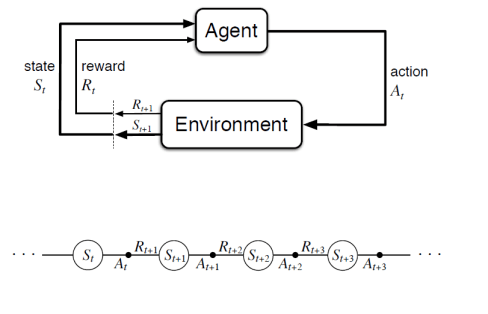
\includegraphics[scale=0.7]{img/rl_base.png}
  \caption{Basic idea of Reinforcement Learning.}
  \label{fig:rl}
\end{figure}

\begin{figure}[h!]
  \centering
  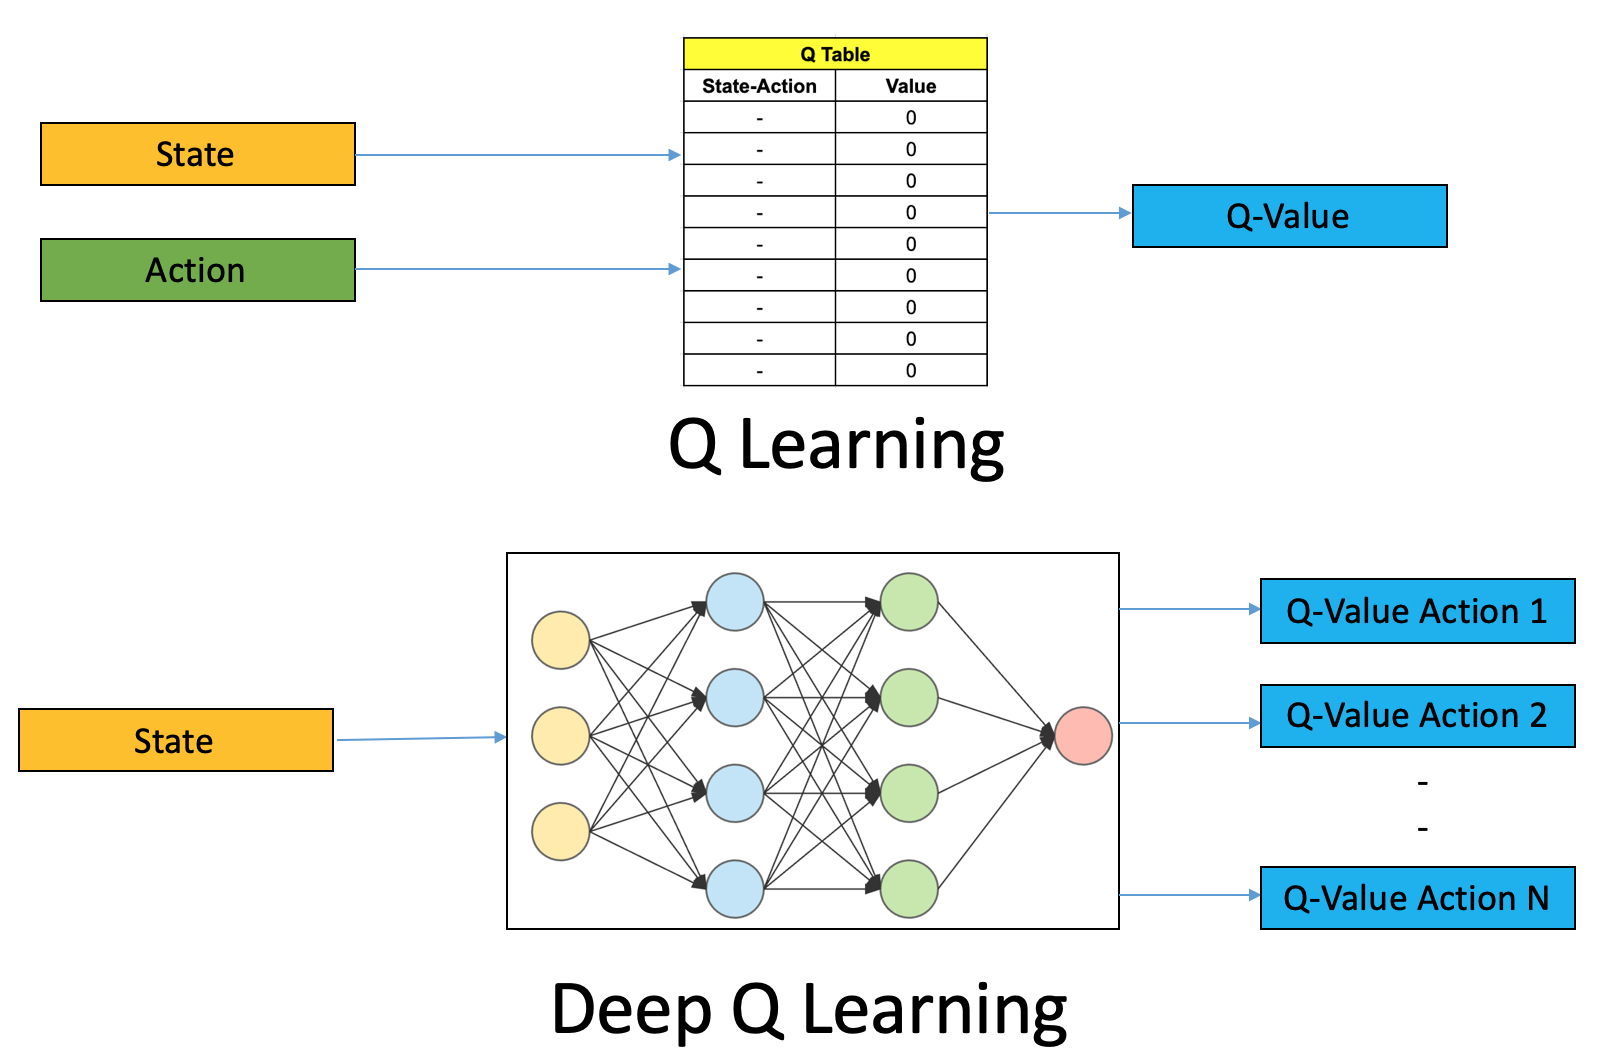
\includegraphics[scale=0.5]{img/dql.png}
  \caption{Basic idea of Reinforcement Learning.}
  \label{fig:dql}
\end{figure}


\subsection{Environment} \label{env}
In the first steps we apply a more simplified environment, which for starters only provides an order schedule with delivery windows. The initial goal is thus for the system to learn which orders are most feasible to complete or award most intermediate rewards.\\
We build the environment so that we can have a precision of seconds, while not specifically modelling each second as a discrete time step. The idea is to merge the discrete time into the actual state as a numerical feature, which is incremented in the expected passed time for a processing step. Initially the elapsed time for the intermediate steps is drawn from Gaussian distributions, which can be later extended with application of the distance matrix and real-world data.\\
The environment utilizing most of the complexity behind the task 

Each task $t_k$ will depend on the duration for a sub-step needed to complete order $O=\sum_{i=0}^N k_i$ and will be modelled as $t_k = \mathcal{N}(\mu_k, \sigma_k^2) + \mathcal{U}(a_M,b_M)$. Here the normal distribution $\mathcal{N}$ is given by $\mu_k=d_{ij}$ drawn from a distance matrix representing the distance between machines $M_i$ and $M_j$. The $\sigma_k$ can either be fine-tuned by hand or matched from real recorded robot data. So in other words $\mathcal{N}$ estimates the duration a robot will need to move. For the uniform distribution $\mathcal{U}$ we adapt the values given from the rulebook, which represent random uniform processing time at the specific machine $M$.

\subsection{States} \label{states}
The state space consists of orders, up to 3 products in the pipeline, distance matrix of the machines, availability of machines and current time. While the distance matrix is constant throughout a game, the other parameters are simulating a dynamic real-time environment.\\
Specifically we can represent an order as a vector of $O=\{\mathcal{B}, \mathcal{R}_1, \mathcal{R}_2, \mathcal{R}_3, \mathcal{C}, n, c, d_{start}, d_{end}  \}$, where
\begin{itemize}
  \item $\mathcal{B}$ represents a set of base types
  \item $\mathcal{R}$ is one of up to 3 ring types
  \item $\mathcal{C}$ is the cap type
  \item $n$ is the requested amount
  \item $c$ indicates whether the order is competitive
  \item $d_{start}$ is the start of the delivery window
  \item $d_{end}$ is the end of the delivery window
\end{itemize}
A intermediate product will look like $\{\mathcal{B}, \mathcal{R}_1, \mathcal{R}_2, \mathcal{R}_3\}$, which corresponds to the physical object one of the 3 robots can transport. We can also omit the cap as we will deliver straight after.\\
The distance matrix and 

While there is still room for changes the current dimensions are 


\subsection{Actions}
The actions 


\subsection{Rewards}
The rewards will be currently 


\subsection{Risk mitigation} \label{risks}
\begin{itemize}
  \item If we need to reduce complexity or in contrast intertwine the actual robot movement deeper into the model, we can apply similar multi-skill and multi-machine approaches as described in \cite{qu2016optimized}.
  \item In the case where the estimation of time consumption for the specific tasks do not represent the real world well enough, we can train an additional neural network in a supervised manner. Here the inputs would be from measured data for given machine distance matrix - to give us more accurate estimations for the expected time consumption at a specific task.
\end{itemize}

\vspace{24pt}

\bibliographystyle{alpha}
\bibliography{description.bib}

\end{document}
